\chapter{Impl\'ementation de la solution}

\section{Introduction}

Ce chapitre aborde comme sujet les choix technologiques et les outils pour l'impl\'ementation de notre solution ainsi que les captures d'\'ecran des diff\'erents fen\^etre r\'ealiser et les tests de validation effectu\'es sur les modules d\'evelopp\'es.

\section{Environnement logiciel}
L'environnement logiciel utilis\'e pour la r\'ealisation de notre projet est pr\'esent\'e dans le tableau suivant :

\begin{table}[H]
\begin{center}
\begin{tabularx}{\textwidth}{ |l|X| }
\hline Outil & Description \\\hline \hline
JDK 1.8 & Java Development Kit (JDK) d\'esigne un ensemble de biblioth\`eques logicielles de base du langage de programmation Java.\\ \hline
Intellij IDEA & Environnement de d\'eveloppement int\'egr\'e (IDE).\\ \hline
Visual Studio Code & Environnement de d\'eveloppement c\^ote frontend.\\ \hline
Android Studio & Environnement de d\'eveloppement pour d\'evelopper des applications mobiles Android.\\ \hline
GitBash & C'est une ligne de commande dans laquelle on peut ex\'ecuter les commandes git.\\ \hline
Zeplin & C'est un outil de design des fonctionnalit\'es. Permet de collaborer entre les designers et les d\'eveloppeurs frontends, facile, efficace et permet de gagner du temps.\\ \hline
Postman & Est actuellement l'un des outils les plus populaires utilis\'es dans les tests d'\gls{API}.\\
\hline
\end{tabularx}
\caption{Environnement logiciel}
\end{center}
\end{table}

\section{Architecture technique du syst\`eme}

Notre syst\`eme se base en totalit\'e sur l'architecture orient\'e service et plus pr\'ecis\'ement sur l'architecture \gls{REST}. C'est un style d'architecture pour la conception d'applications faiblement coupl\'ees sur \gls{HTTP}, souvent utilis\'e dans le d\'eveloppement de services Web.

Une \'etude qui a \'et\'e faite par l'entit\'e \gls{DF}, ils sont convaincu d'adapter quelques technologies qu'on va les utiliser. La figure suivante repr\'esente les technologies utilises dans notre projet.

\begin{figure}[H]
	\center{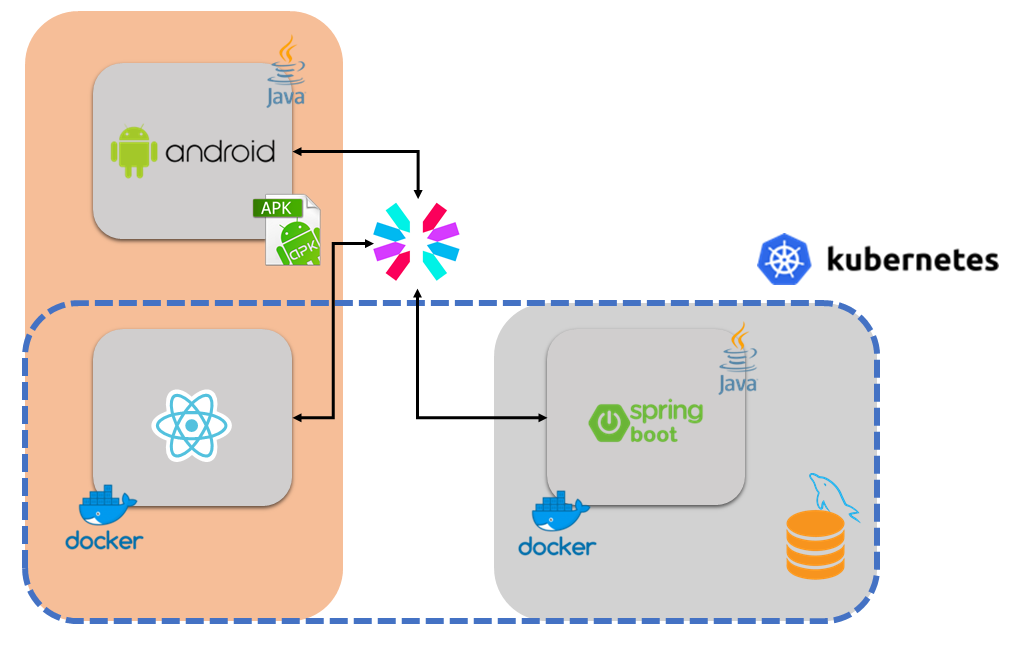
\includegraphics[width=\textwidth]{Figures/achitec-tech.PNG}}
	\caption{\label{fig:my-label} Architecture technique du syst\`eme}
\end{figure}

Maintenant, on va expliquer l'utilit\'e des technologies utilises dans notre impl\'ementation. 

